\documentclass[journal]{IEEEtran}

\ifCLASSINFOpdf
  
\else
  
\fi
\raggedbottom

\hyphenation{op-tical net-works semi-conduc-tor}

\usepackage[numbers,sort&compress]{natbib}
\usepackage{xurl}
\usepackage{array}
\usepackage{graphicx}
\usepackage{amsmath}
\usepackage{amssymb}
\usepackage{booktabs}
\usepackage{multirow}
\usepackage{algorithm, algorithmic}
\usepackage{float}

\begin{document}

\title{HiLTL: Hierarchical Temporal Logic Integration for LTL Satisfaction in Reinforcement Learning}


\author{Anonymous Authors%
\thanks{Anonymous Institution, Under Review}}

% The paper headers
% Running header will follow the selected journal template.

% make the title area
\maketitle

% As a general rule, do not put math, special symbols or citations
% in the abstract or keywords.
\begin{abstract}
Learning policies that satisfy Linear Temporal Logic (LTL) specifications requires representations of task structure and estimates of long-horizon return. We propose HiLTL, a hierarchical neuro-symbolic framework that augments reach--avoid sequence conditioning with semantically enhanced graph neural networks and a Long--Short Term Fusion architecture. The graph encoder represents automaton node roles, transition types, and guards. Two value pathways use temporal-difference (TD) and Monte Carlo (MC) supervision, and a fixed sigmoid gate varies their weights with automaton proximity. The reported aggregate ZoneEnv comparison gives a +6.4\% relative success-rate improvement over the internal baseline. Cross-environment comparisons and component ablations provide further descriptive evidence for the value-learning design on the tested logic-conditioned control tasks.
\end{abstract}

% Note that keywords are not normally used for peerreview papers.
\begin{IEEEkeywords}
LTL Specification, Reinforcement Learning, Graph Neural Networks, Neuro-Symbolic AI, Automata, Long--Short Term Fusion.
\end{IEEEkeywords}






% For peer review papers, you can put extra information on the cover
% page as needed:
% \ifCLASSOPTIONpeerreview
% \begin{center} \bfseries EDICS Category: 3-BBND \end{center}
% \fi
%
% For peerreview papers, this IEEEtran command inserts a page break and
% creates the second title. It will be ignored for other modes.
\IEEEpeerreviewmaketitle



\section{Introduction}

\IEEEPARstart{T}{he} integration of formal methods with reinforcement learning provides a principled foundation for developing verifiable and safe autonomous systems~\citep{Baier2008}. Linear Temporal Logic (LTL)~\citep{Pnueli1977} serves as a powerful specification language for expressing complex temporal requirements: safety constraints (e.g., never entering forbidden regions), liveness goals (e.g., eventually reaching targets), and sequential ordering constraints (e.g., visiting locations in a specific order). A central challenge is zero-shot generalization, i.e., training agents on a limited set of LTL specifications and ensuring they can satisfy completely unseen formulas without retraining.

Graph-based automaton representations support reusable task-conditioned policies~\citep{Yalcinkaya2024}. DeepLTL~\citep{deepltl} provides a strong baseline based on reach--avoid sequence conditioning and automaton-based sequence selection. HiLTL retains this backbone and augments it with semantic graph context and progress-gated value learning.

Figure~\ref{fig:limitations} motivates two design goals. (1) Explicit transition semantics: node roles, progress transitions, non-progress transitions, and epsilon choices provide structural context beyond untyped topology. (2) Progress-conditioned value learning: environmental observations and logical context provide complementary information for estimating discounted return. HiLTL addresses these goals through semantic graph features, TD/MC value supervision, and a fixed progress-dependent fusion rule.

\begin{figure*}[t]
\centering
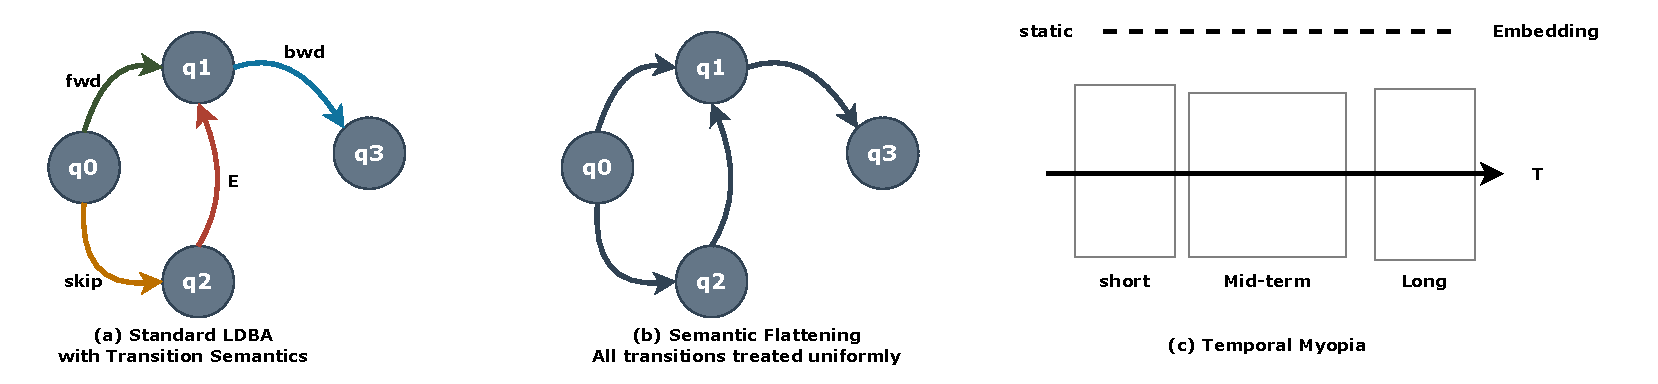
\includegraphics[width=0.95\linewidth]{figure_limitations.pdf}
\caption{\textbf{Design motivations.} The figure illustrates transition roles and the limitations of omitting task structure and temporal context. The displayed edge labels describe qualitative roles. The operative classifier uses progress, remaining non-epsilon transitions, and epsilon choices, with the skip slot reserved as specified in Eq.~\ref{eq:transition_types}. TD- and MC-supervised value pathways are combined through progress-dependent fusion.}
\label{fig:limitations}
\end{figure*}

This study proposes HiLTL, shown in Figure~\ref{fig:architecture}, with three components: (1) Semantically-Enhanced GNNs (SE-GNN) injecting transition type and node role signals; (2) hierarchical value learning with TD- and MC-supervised pathways; and (3) fixed sigmoid fusion whose weight varies with automaton progress.

\section{Related Work}
\label{sec:related}

Neuro-symbolic RL integrates formal methods with neural policies~\citep{Jothimurugan2021}. LTL~\citep{Pnueli1977,Baier2008} can be translated into LDBAs~\citep{Sickert2016}; our implementation uses Rabinizer~\citep{Rabinizer2018}. DeepLTL~\citep{deepltl} provides a strong baseline using reach--avoid sequence conditioning. Related LTL-RL approaches~\citep{Vaezipoor2021,Hahn2021,bozkurt2020control} and reward-machine methods~\citep{Icarte2022,Toro2020} expose logical task structure through different interfaces. General graph architectures~\citep{Kipf2017,Gilmer2017} motivate representation learning, while HiLTL focuses on explicit automaton features and progress-dependent value fusion.

LTL2Action~\citep{Vaezipoor2021} learns formula-conditioned policies for multi-task control. GCRL-LTL~\citep{Qiu2023} combines goal-conditioned reinforcement learning with temporal-logic objectives. Both provide external methodological references; the internal DeepLTL comparison isolates changes within the inherited sequence-conditioning backbone.

Recent advances in GNN expressiveness~\citep{Dwivedi2023,sato2020survey,ying2021transformers,morris2019weisfeiler} and classic inductive message passing~\citep{Hamilton2017} provide complementary perspectives on structural encoding. Graph matching networks~\citep{li2019graph} further highlight the value of similarity-aware graph representations when structure matters across instances. Hierarchical RL~\citep{Sutton2018,Bacon2017,Nachum2018,Vezhnevets2017} learns or specifies temporal abstractions, while LTL automata expose task structure explicitly. Logic-guided RL~\citep{HasanbeigCertified2021} and neural-network verification~\citep{katz2017reluplex} address complementary aspects of correctness, while non-Markovian rewards~\citep{Gaon2020} and interpretable policy learning~\citep{glanois2024survey} explore related formalisms.

\subsection{Comparative Positioning}

Reward-machine approaches~\citep{IcarteRewardMachines2019,Icarte2022} expose task structure through reward specifications and automaton state. HiLTL instead focuses on TD- and MC-supervised value pathways and progress-dependent fusion, while retaining the inherited task rewards. Its contribution is this value-learning architecture rather than automaton tracking alone.

Hierarchical RL~\citep{Bacon2017,Nachum2018} uses temporal abstractions such as options. HiLTL uses explicit automaton structure to condition value learning. Automaton states provide logical context, and distance to accepting-transition targets provides a structural proximity signal; neither implies that every state transition advances toward acceptance.

\begin{figure*}[t]
\centering
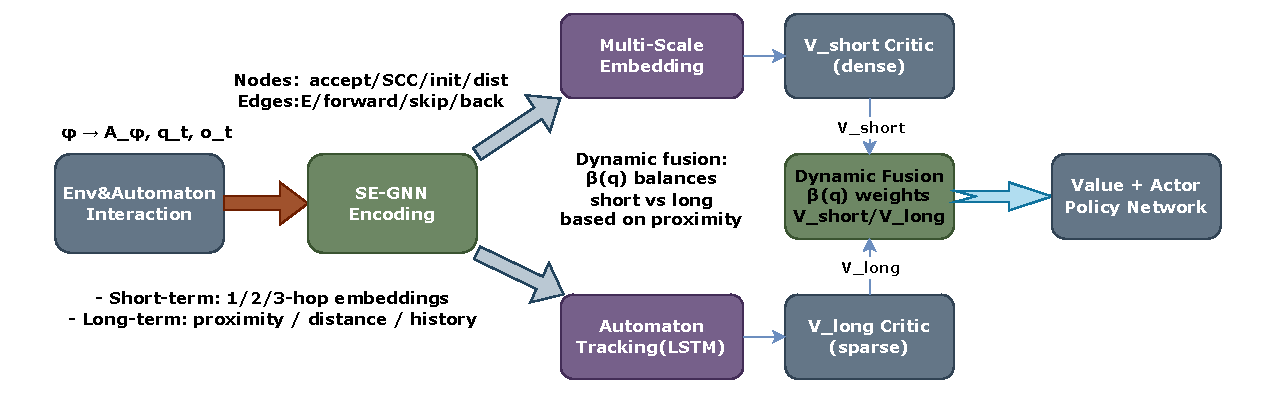
\includegraphics[width=0.95\linewidth]{figure6_architecture.pdf}
\caption{HiLTL architecture with all representation components shown. SE-GNN encodes automaton features and guards. Multi-layer pooling and history encoding are enabled by configuration. The two value pathways use TD and completed-episode MC supervision, respectively, and a fixed progress-dependent gate fuses their scalar estimates. The actor has a separate output path conditioned on environmental and task representations; the fused value supplies the critic used by PPO. The edge labels and dense/sparse labels in the diagram are schematic.}
\label{fig:architecture}
\end{figure*}

\section{Preliminary}
\label{sec:problem}

\subsection{Problem Formulation}

We seek a policy that maximizes the probability of satisfying an LTL specification $\varphi$. Let $AP$ be the atomic propositions and $L:S\to2^{AP}$ the labeling map. The environment MDP is $\mathcal M=(S,A,P,R,\gamma_{\mathrm{RL}})$ and the transition-accepting LDBA is $\mathcal A_\varphi=(Q,2^{AP},\delta,q_0,F_E)$, with epsilon choices handled explicitly. Here $F_E$ is the set of accepting transitions. The product state is $(s,q)\in S\times Q$. The task-level objective is:
\begin{equation}
\pi^* = \arg\max_\pi \Pr[\text{formula } \varphi \text{ is satisfied}]
\label{eq:opt_policy}
\end{equation}
B\"uchi acceptance requires infinitely many accepting transitions along an infinite run. Training uses the inherited discounted reward objective as a surrogate. We define the return value as:

\begin{equation}
V^\pi(s,q) = \mathbb{E}^\pi\left[\sum_{t=0}^\infty \gamma_{\text{RL}}^t r_t \mid s_0 = s, q_0 = q\right]
\label{eq:value_func}
\end{equation}
Here $\pi(a\mid s,q)$ is a stochastic policy over product states $(s,q)$, and $P(s'\mid s,a)$ is the environment transition kernel. Rewards $r_t$ include the inherited environment and task rewards on the product trajectory. The value $V^\pi(s,q)$ is the expected discounted return starting from $(s,q)$ under $\pi$, with discount $\gamma_{\text{RL}} \in (0,1)$.

\textbf{Key notation.} Labels satisfy $L(s_t)\in2^{AP}$, and enabled transitions determine successor logical states, including explicit epsilon choices. Define $Q_F=\{q':(q,\ell,q')\in F_E\}$ and let $d(q)$ be the shortest directed hop distance from $q$ to $Q_F$, with $d(q)=\infty$ when no path exists. Set
\begin{equation*}
\begin{aligned}
D&=\max\!\left(1,\max_{q:d(q)<\infty}d(q)\right),\\
\bar d(q)&=\frac{\min\{d(q),D\}}{D},\qquad p(q)=1-\bar d(q).
\end{aligned}
\end{equation*}
The inner maximum of an empty set is zero. Unreachable states have $\bar d(q)=1$ and $p(q)=0$. In subsequent distance notation, $\operatorname{dist}(q,F)$ denotes $d(q)$ and $\operatorname{max\_dist}$ denotes $D$; this legacy $F$ refers to $Q_F$, not $F_E$. Also $\operatorname{proximity}(q)=p(q)$. These are structural distances rather than physical travel times. Graph and history arguments of value functions are implicit unless needed.

\subsection{Structural Context in LDBAs}
We distinguish three effective transition categories:
\begin{equation}
\mathcal T_{\mathrm{active}}=\{\tau_{\mathrm{progress}},\tau_{\mathrm{remaining}},\tau_\epsilon\}.
\label{eq:transition_types}
\end{equation}
Epsilon transitions are classified first. A non-epsilon edge $(q,\ell,q')$ is classified as progress if $d(q')<d(q)$ and as remaining otherwise. The remaining category includes self-loops, equal-distance edges, and edges leading away from $Q_F$; it is not restricted to accepting cycles. The four-slot type vector retains a zero skip slot for compatibility. Under shortest-hop distance, a real single edge cannot decrease distance by more than one, so this slot is not presented as an observed multi-hop shortcut.

\subsection{Hierarchical Value Parameterization}
We parameterize the fused critic by a convex combination:
\begin{equation}
V(s,q)=(1-\beta(q))V_{\mathrm{short}}(s,q)+\beta(q)V_{\mathrm{long}}(s,q).
\label{eq:decomposition}
\end{equation}
The two pathways use different inputs and supervision. Their targets and gate are
\begin{align*}
y_t^{\mathrm{short}}&=r_t+\gamma_{\mathrm{RL}}(1-m_t)
 \operatorname{stopgrad}\!\left[V_{\mathrm{short}}(s_{t+1},q_{t+1})\right],\\
G_t&=\sum_{k=t}^{T-1}\gamma_{\mathrm{RL}}^{k-t}r_k,\\
\beta(q)&=\sigma\!\left(\kappa(p(q)-\theta)\right),\qquad\kappa=3,\quad\theta=0.5.
\end{align*}
Here $m_t$ is the episode-end mask and $T$ is the number of transitions in a completed episode. The short head is trained against $y_t^{\mathrm{short}}$; the long head predicts $G_t$ from environmental and logical context. Negative rewards are retained. Both heads concern discounted return: one-step TD supervision does not imply a one-step prediction horizon. The long head is a return surrogate rather than a calibrated satisfaction probability. The names short and long distinguish input and supervision pathways rather than an exact additive decomposition of rewards. The fixed gate gives $\beta\in[0.1824,0.8176]$ approximately for $p\in[0,1]$. Its weight varies with logical progress rather than training time, and progress need not be monotone. Figure~\ref{fig:fusion_overview} illustrates the two pathways.

\begin{figure*}[t]
\centering
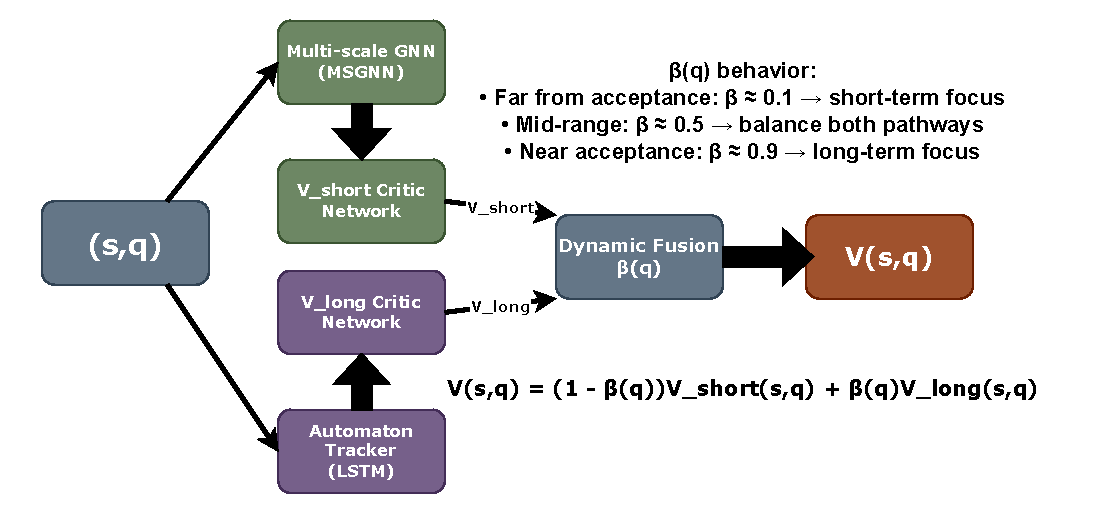
\includegraphics[width=0.95\linewidth]{figure2_fusion.pdf}
\caption{Fusion overview. Both pathways use environmental and logical context. The short head uses one-step TD supervision, and the long head uses completed-episode discounted returns and optional visited-state history. Multi-layer pooling, when enabled, provides context from three message-passing depths. The fixed sigmoid in Eq.~\ref{eq:beta_definition} combines the estimates as $V=(1-\beta)V_{\mathrm{short}}+\beta V_{\mathrm{long}}$. The curve in Figure~\ref{fig:fusion_weight} gives endpoint weights of approximately 0.1824 and 0.8176.}
\label{fig:fusion_overview}
\end{figure*}

\section{Methodology}
\label{sec:method}

\subsection{Overview of Proposed Approach}

As shown in Figure~\ref{fig:automaton_enhanced}, HiLTL combines three elements. First, SE-GNN encodes node roles and transition semantics through edge-conditioned GATv2 attention; its four-slot type vector contains three effective categories and a reserved skip slot. Second, TD- and MC-supervised value pathways are combined by the fixed progress-dependent sigmoid in Eq.~\ref{eq:beta_definition}. Third, when enabled, multi-layer pooling combines representations from one-, two-, and three-hop message-passing depths, providing structural context rather than fixed physical planning horizons.

%These components integrate into the architecture in Figure~\ref{fig:automaton_enhanced}.

\begin{figure*}[t]
\centering
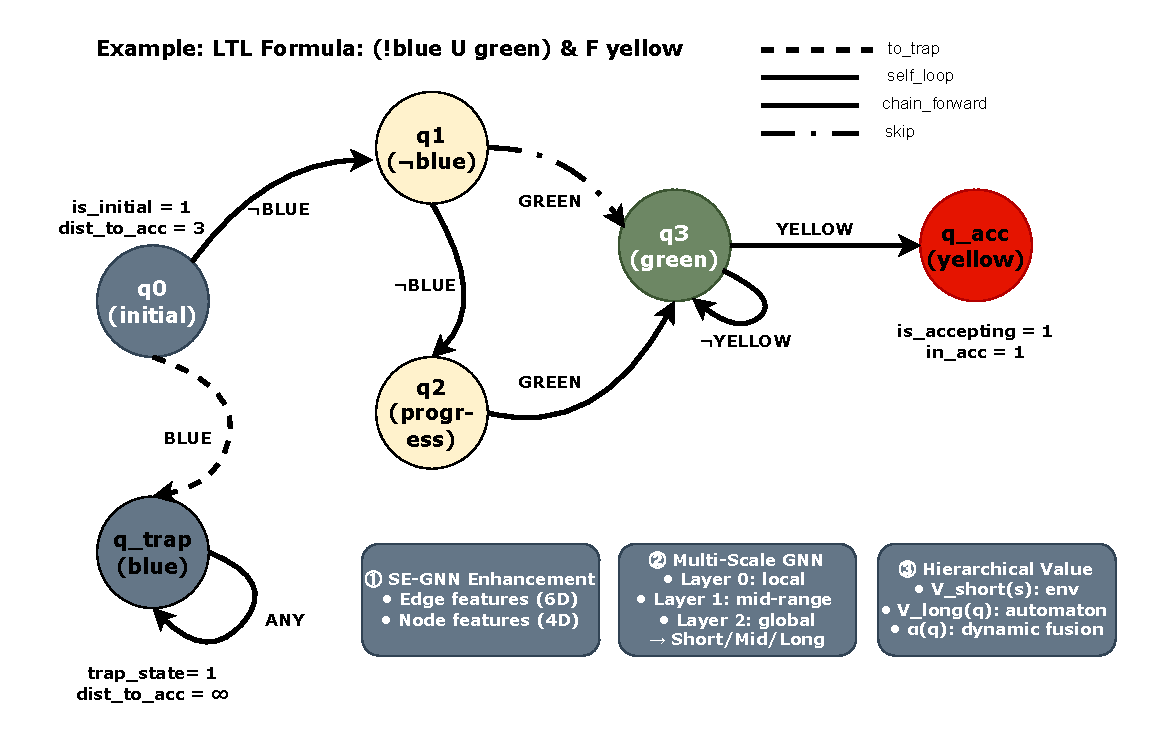
\includegraphics[width=0.95\linewidth]{figure_automaton_enhanced.pdf}
\caption{Conceptual illustration of automaton features motivated by $(\neg\mathrm{blue}\mathrel U\mathrm{green})\land F\mathrm{yellow}$. The displayed paths are a partial illustration, not a complete language-equivalent translation of this formula or a full B\"uchi acceptance structure. Four-dimensional node features encode targets of accepting transitions, cyclic-SCC membership, the initial state, and normalized distance. Six-dimensional edge features are defined in Eq.~\ref{eq:edge_features}; illustrative edge names do not replace that classifier. Three GNN layers provide one-, two-, and three-hop context, without guaranteeing global information at every node. The value pathways use a fixed progress-dependent gate. Acceptance is defined on transitions.}
\label{fig:automaton_enhanced}
\end{figure*}

\subsection{Semantically-Enhanced Graph Neural Networks}

\subsubsection{Graph Structure of Automaton}

Node and edge features encode automaton structure. For an infinite trace $\rho$, $\rho\models\varphi$ denotes LTL satisfaction. A trap state has no accepting continuation. Define
\begin{equation}
\label{eq:node_features}
h_v(q)=[\mathbb I(q\in Q_F),\mathbb I(q\in C),\mathbb I(q=q_0),\bar d(q)],
\end{equation}
where $C$ is the set of states lying on a directed cycle: its SCC has more than one state or the state has a self-loop. Membership in $Q_F$ is a structural feature and does not replace transition-based B\"uchi acceptance.

For an edge $e=(q,\ell,q')$, the structural feature vector is
\begin{equation}
\label{eq:edge_features}
\begin{split}
h_e(e)=[&\mathbb I(\mathrm{progress}),\mathbb I(\mathrm{remaining}),0,\\
        &\mathbb I(\epsilon),\mathbb I(q'\in Q_F),\bar d(q')].
\end{split}
\end{equation}
Classification follows the epsilon-first rule above. The third type slot is reserved and remains zero; every edge has exactly one active type indicator. The last component is the target's normalized distance, not an absolute distance difference. Transition guards are encoded separately and combined with the structural vector for edge-conditioned attention. No category is assigned a fixed positive or negative attention contribution.

\subsubsection{Semantically-Conditioned GATv2 Mechanism}

An attention score without edge features can be written as follows~\citep{Brody2022}:
\begin{equation}
\label{eq:gat_standard}
e_{ji}^{\mathrm{standard}}=\mathbf a^\top\operatorname{LeakyReLU}
 (W_s\mathbf h_j+W_t\mathbf h_i).
\end{equation}
We use the edge-feature interface of GATv2 to incorporate automaton semantics. For an incoming edge $j\to i$,
\begin{align}
\label{eq:gat_semantic}
e_{ji}&=\mathbf a^\top\operatorname{LeakyReLU}
 (W_s\mathbf h_j+W_t\mathbf h_i+W_e\mathbf e_{ji}),\\
\alpha_{ji}&=\frac{\exp(e_{ji})}{\sum_{k:(k,i)\in E}\exp(e_{ki})},
\end{align}
where $\mathbf e_{ji}$ combines the structural edge features and guard encoding.
Edge features allow the network to learn transition-dependent attention weights. A progress indicator does not guarantee a positive contribution or a larger score. For a fixed graph and parameters, graph attention does not change solely because the agent's current state changes; progress conditioning enters through current-node features, optional history, and the value gate.

\subsubsection{SE-GNN Architecture Details}

The SE-GNN consists of three GATv2 layers with residual connections~\citep{He2016} and layer normalization~\citep{Ba2016}, as specified below. Graph transformers~\citep{rampavsek2022recipe} and message-passing PDE solvers~\citep{brandstetter2022message} provide broader architectural context:
\begin{align}
\mathbf u^{(l+1)} &= \operatorname{GATv2}
 (\mathbf x^{(l)},E,\mathbf e),\\
\mathbf x^{(l+1)} &= \operatorname{LayerNorm}
 \bigl(\mathbf x^{(l)}+\operatorname{MLP}_l(\mathbf u^{(l+1)})\bigr).
\end{align}
We use three GATv2 layers with four attention heads, residual connections, and LayerNorm. Before graph-level pooling, the layers provide at most one-, two-, and three-hop directed message-passing context. Pooling summarizes node representations, while current-node features condition subsequent prediction. Three hops do not in general give each node global relational information, and graph distance is not a fixed number of physical control steps.

\subsection{MSGNN for Short-Term Features}

The short-term value network uses environmental observations and graph context to estimate discounted return under one-step TD supervision. When multi-layer pooling is enabled, it combines embeddings from the SE-GNN layers.
We extract embeddings at three aggregation levels,
\begin{equation}
\mathbf{z}^{(l)}_{\text{pool}} = \text{ReadOut}(\mathbf{H}^{(l)}) \quad \text{for } l = 1, 2, 3
\label{eq:multiscale_readout}
\end{equation}
where ReadOut is learnable global attention pooling:
\begin{equation}
\label{eq:readout}
	\text{ReadOut}(\mathbf{H}) = \sum_{i=1}^{n} \text{softmax}_i(\mathbf{w}^T \text{ReLU}(\mathbf{W}_{\text{pool}} \mathbf{h}_i)) \cdot \mathbf{h}_i,
\end{equation}
where $\mathbf H=\{\mathbf h_1,\ldots,\mathbf h_n\}$ is the node representation set, and $\mathbf w$ and $\mathbf W_{\mathrm{pool}}$ are learnable parameters. Softmax weights sum to one, giving a graph-level weighted sum. The layers correspond to message-passing depths rather than fixed physical-time horizons. With multi-layer pooling enabled, the representation is
\begin{equation}
\mathbf{z}_{\text{short}} = [\mathbf{z}_{\text{pool}}^{(1)}; \mathbf{z}_{\text{pool}}^{(2)}; \mathbf{z}_{\text{pool}}^{(3)}],
\end{equation}
and the short-term value function processes the combined representation with the current environment state
\begin{equation}
V_{\text{short}}(s, q) = \text{MLP}_{\text{short}}([\mathbf{s}, \mathbf{z}_{\text{short}}, \mathbf{z}_{\text{GNN}}(q)]),
\label{eq:short_value_comp}
\end{equation}
Here $\mathbf s$ encodes the environment state, and $\mathbf z_{\mathrm{GNN}}(q)$ is the current-node embedding. For configurations without multi-layer pooling, $\mathbf z_{\mathrm{short}}$ is replaced by the final-layer pooled representation. The implementation may retain the inherited DeepLTL critic as a residual baseline; this does not change the TD/MC supervision distinction.

\subsection{Automaton Tracking for Long-Term Features}

We use three logical-context signals. (1) Directed distance $d(q)$ is computed by reverse multi-source BFS from $Q_F$, including explicit epsilon edges. (2) History $H_t=[q_0,\ldots,q_t]$ records visited logical states, including repetitions, and is encoded by an LSTM when tracking is enabled. It is reset with the episode and updated on real interaction steps rather than repeated forward passes. (3) Proximity is $p(q)=1-\bar d(q)$, using the normalization and unreachable-state convention above.

The long head aggregates environmental and logical-context signals:
\begin{equation}
V_{\mathrm{long}}(s_t,q_t)=\operatorname{MLP}_{\mathrm{long}}
 ([\mathbf s_t;p(q_t);\mathbf h_{q_t};\operatorname{Enc}(H_t)]).
\end{equation}
Here $\mathbf s_t$ encodes the environment state. The graph and optional history are implicit arguments; without tracking, the history term is omitted. The head predicts completed-episode discounted return. Distance is a structural prior rather than a physical difficulty estimate; higher proximity gives higher gate weight, but neither must increase monotonically within a trajectory.

\begin{table}[t]
\centering
\caption{Evaluation Configuration Matrix}
\label{tab:configurations}
\small
\begin{tabular}{@{}lcccc@{}}
\toprule
\textbf{Configuration} & \textbf{HV} & \textbf{MSGNN} & \textbf{Track} & \textbf{Options} \\ \midrule
baseline & $\times$ & $\times$ & $\times$ & $\times$ \\
hv\_only & \checkmark & $\times$ & $\times$ & $\times$ \\
msgnn\_only & $\times$ & \checkmark & $\times$ & $\times$ \\
hv\_track & \checkmark & $\times$ & \checkmark & $\times$ \\
msgnn\_track & $\times$ & \checkmark & \checkmark & $\times$ \\
full\_no\_options & \checkmark & \checkmark & \checkmark & $\times$ \\
full\_all & \checkmark & \checkmark & \checkmark & \checkmark \\ \bottomrule
\end{tabular}
\end{table}
\noindent\textit{Configuration scope.} HV denotes the dual value heads and fixed progress gate; MSGNN denotes concatenation of pooled representations from multiple layers; Track denotes encoding visited logical-state history. Enhanced variants retain a semantic graph encoder even when MSGNN is disabled. The Options-enabled row is a historical reference outside the six configurations supported by the maintained implementation and is excluded from controlled component-level conclusions.

\subsection{Dynamic Fusion with Adaptive Weighting}

The fusion rule adjusts the relative weights of the TD- and MC-supervised heads according to automaton proximity:
\begin{equation}
\beta(q)=\sigma\!\left(\kappa(p(q)-\theta)\right),\qquad
\kappa=3,\quad\theta=0.5.
\label{eq:beta_definition}
\end{equation}
Here $p(q)=\operatorname{proximity}(q)=1-\bar d(q)$ and $\sigma$ is the logistic sigmoid. The gate constants are fixed, with $\beta=0.5$ at $p=0.5$. The reward discount is denoted $\gamma_{\mathrm{RL}}$.

At $p=0$, $\beta=\sigma(-1.5)\approx0.1824$; at $p=0.5$, $\beta=0.5$; and at $p=1$, $\beta=\sigma(1.5)\approx0.8176$. Higher proximity therefore increases the logical-context head's contribution. Smoothness in proximity does not imply continuous actions or policies along discrete automaton transitions.

\section{Experiments}
\label{sec:experiments}

\subsection{Experimental Setup}

	\textbf{Model parameters and reported protocol.} The SE-GNN uses three GATv2 layers with 64-dimensional outputs, four attention heads, LayerNorm, and LeakyReLU ($\alpha=0.2$). Node and structural edge features have dimensions four and six, respectively; guards are encoded separately. The short and long heads each use two hidden layers, of widths 256 and 128, respectively, followed by a scalar output. Both pathways receive environmental and logical context, and the long pathway optionally receives history. The gate is fixed at $\kappa=3$ and $\theta=0.5$. The reported experiments use PPO~\citep{Schulman2017}, Adam~\citep{Kingma2015}, 1{,}000{,}000 training timesteps, minibatches of 64, and learning rate $3\times10^{-4}$. The reported ZoneEnv discount is $\gamma_{\mathrm{RL}}=0.998$. Advantages are clipped to $[-1,1]$ before the actor update; this is separate from PPO's probability-ratio clipping. Evaluation means are reported over seeds 1--5 with 500 episodes per seed. The internal baseline follows the DeepLTL architecture~\citep{deepltl}; enhanced configurations add the components specified in Table~\ref{tab:configurations}.

	\textbf{Environments and tasks.} We compare PointLtl2-v0 (ZoneEnv), LetterEnv, and FlatWorld. ZoneEnv uses continuous actions; the evaluated LetterEnv and FlatWorld variants use discrete actions. Table~\ref{tab:tasks} gives the three finite-task templates for ZoneEnv and FlatWorld. For LetterEnv, blue, green, and yellow are replaced by $a$, $b$, and $c$, respectively. Recurrent and persistence objectives are illustrated by finite trajectory excerpts in Figure~\ref{fig:zoneenv_vis}. The reported configurations are listed in Table~\ref{tab:configurations}.

    \textbf{External baselines}: To broaden comparison beyond internal ablations, we additionally include LTL2Action~\citep{Vaezipoor2021} and GCRL-LTL~\citep{Qiu2023} in the main performance table and cross-environment analyses. External baseline values are retained from the original DeepLTL study and are reported as historical reference results; internal comparisons use our evaluation pipeline.

\begin{table}[htbp]
\centering
\caption{Task Evaluation Set}
\label{tab:tasks}
\resizebox{0.9\linewidth}{!}{%
\begin{tabular}{@{}lp{5.5cm}@{}}
	\toprule
	\textbf{Property} & \textbf{Value} \\ \midrule
	\textbf{Task $\varphi_1$} & \\
\quad Formula & $F\,\text{blue} \land F\,\text{green}$ \\
\quad Difficulty & Easy \\
\quad LDBA Size & 5 states \\
\quad Type & Conjunctive reachability \\ \midrule
	\textbf{Task $\varphi_2$} & \\
\quad Formula & $(F\,\text{blue}) \land (F\,\text{green}) \land (F\,\text{yellow})$ \\
\quad Difficulty & Medium \\
\quad LDBA Size & 12 states \\
\quad Type & Aggregation \\ \midrule
	\textbf{Task $\varphi_3$} & \\
\quad Formula & $(\neg\,\text{blue}\ U\ \text{green}) \land F\,\text{yellow}$ \\
\quad Difficulty & Hard \\
\quad LDBA Size & 18 states \\
\quad Type & Constraint \\ \bottomrule
\end{tabular}
}
\end{table}
\noindent\textit{Automaton counts.} State counts in Table~\ref{tab:tasks} refer to the reported experiments and depend on translation and simplification. The current maintained code produces 4, 8, and 5 states for the corresponding templates after legal-valuation pruning; these are different conversion artifacts, not replacements for the historical counts.

	\textbf{Evaluation metrics.} SR denotes the proportion of completed test episodes satisfying a finite-task objective. Reported evaluation means use seeds 1--5 and 500 episodes per seed. Secondary metrics are mean completion steps and cumulative reward. Relative SR gain is $100(\mathrm{SR}_{\mathrm{method}}/\mathrm{SR}_{\mathrm{reference}}-1)\%$; absolute SR differences are reported in percentage points (pp). Derived quantities are calculated from displayed values before rounding. The comparisons below are descriptive; no inferential significance claim is made.

%\textbf{Main-text limitations}: Remaining limitations are discussed in Appendix~\ref{app:future_directions}, focusing on larger-automata scalability.

\begin{table}[htbp]
\centering
\caption{HV-Related Aggregate Configuration Performance}
\label{tab:hv_comparison}
\begin{tabular}{@{}lcc@{}}
\toprule
\textbf{Configuration} & \textbf{Avg SR} & \textbf{Relative gain} \\ \midrule
baseline & 0.933 & --- \\
hv\_only & 0.975 & +4.5\% \\
hv\_track & \textbf{0.993} & \textbf{+6.4\%} \\
full\_all & 0.963 & +3.2\% \\ \bottomrule
\end{tabular}
\end{table}

\subsection{Overall Performance}

\begin{figure*}[t]
  \centering
  % Row 1
  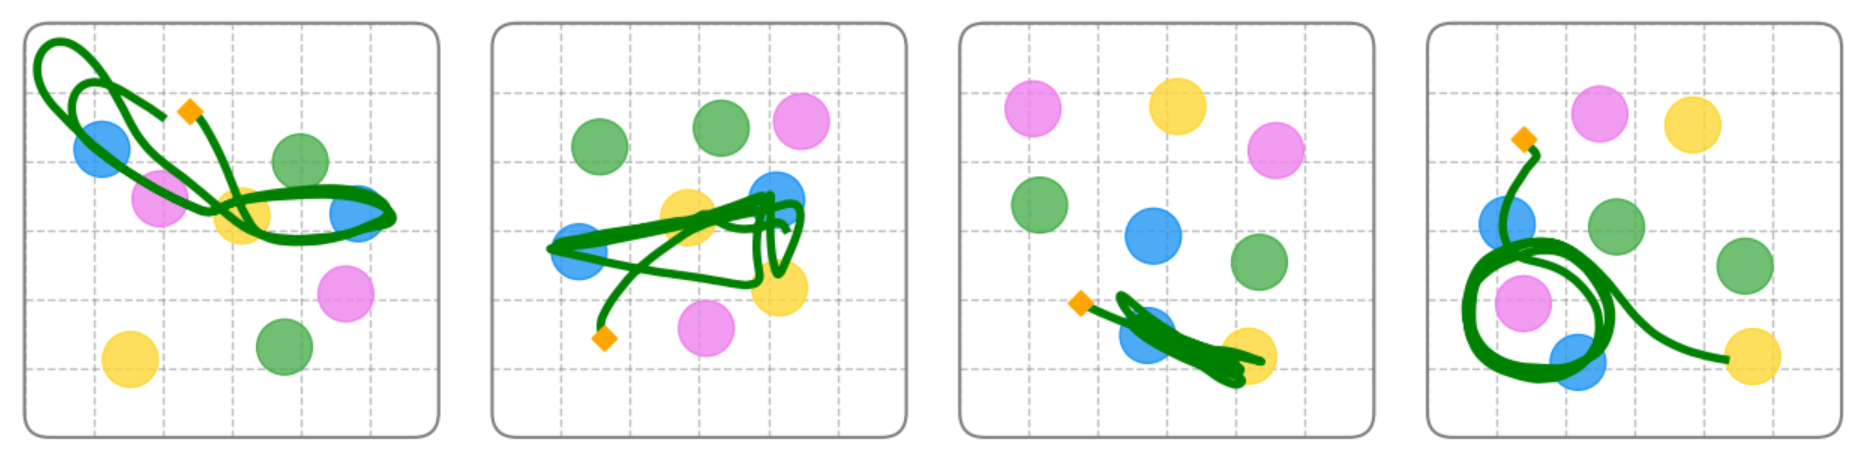
\includegraphics[width=0.95\linewidth]{zoneenv_gFblue_yellow.png.png}
  \vspace{6pt}
  % Row 2
  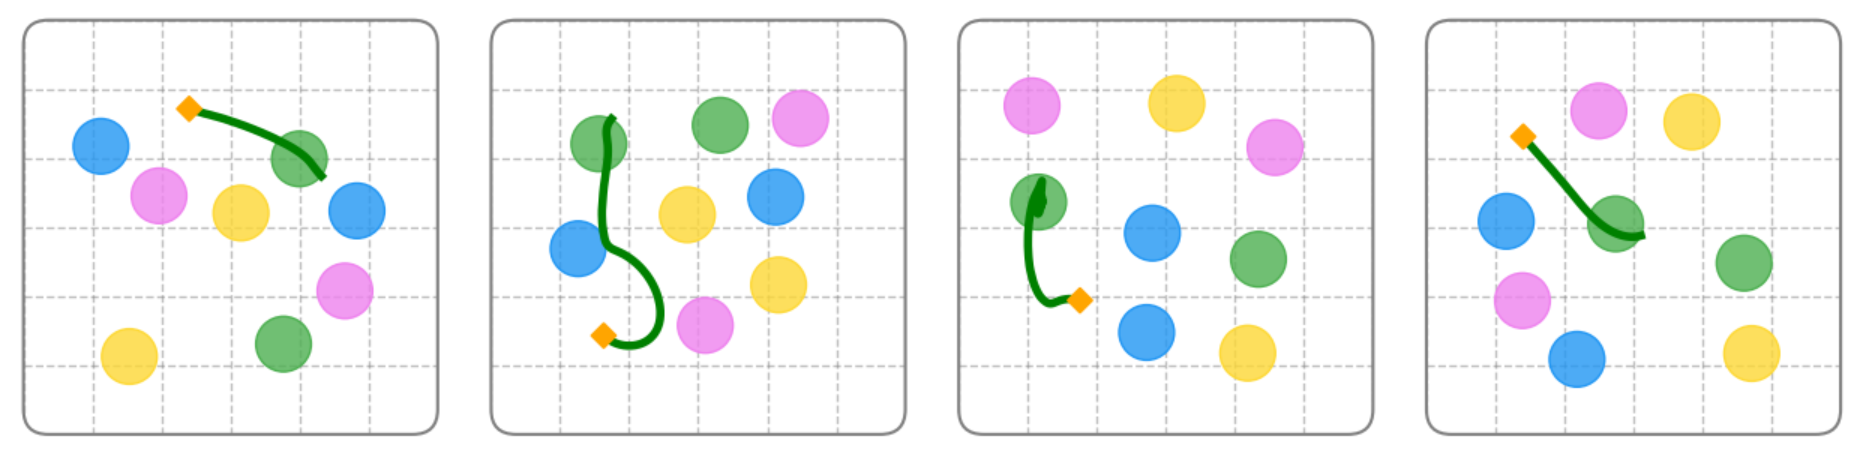
\includegraphics[width=0.95\linewidth]{zoneenv_FGgreen.png.png}
  \vspace{-2pt}
  \caption{ZoneEnv visualization examples under two typical LTL objectives, shown as two rows spanning both columns. Top: $GF\,\mathrm{blue}\land GF\,\mathrm{yellow}$, with repeated visits to blue and yellow regions. Bottom: $FG\,\mathrm{green}$, with residence in the green region over the displayed window. These finite trajectories illustrate behavior and do not establish infinite-horizon satisfaction.}
  \label{fig:zoneenv_vis}
\end{figure*}

The reported aggregate comparison includes seven configurations, with full\_all retained as a historical Options-enabled reference. Figure~\ref{fig:zoneenv_vis} illustrates behavior under recurrent and persistence objectives. In the aggregate comparison, hv\_track achieves 99.3\% SR, corresponding to a +6.4\% relative gain over the internal baseline; hv\_only and msgnn\_only achieve +4.5\% and +2.3\%, respectively. These results motivate investigation of hierarchical value learning. Evaluation on larger automata remains future work.

Table~\ref{tab:overall_performance} summarizes aggregate results. Among the reported internal variants, hv\_track has the highest average SR (0.993) and average reward (0.663), with 235.5 mean steps. The corresponding baseline values are 0.933, 0.618, and 231.3. The hv\_only and msgnn\_only variants improve aggregate SR by +4.5\% and +2.3\%, respectively, while full\_no\_options is 0.4\% below baseline. These means describe configuration-level differences and do not identify a unique optimization mechanism.

The aggregate results favor hierarchical value learning: hv\_track exceeds hv\_only by 1.8 percentage points (0.993 versus 0.975), or approximately 1.85\% relative to hv\_only. Component-removal results are reported in Section~\ref{app:ablation}. Larger-automaton evaluation is discussed in Appendix~\ref{app:future_directions}.

\subsection{External Baseline Coverage}

To strengthen baseline completeness, we complement internal ablations with two representative external families: structure-conditioned policy learning (LTL2Action) and compositional goal-conditioned planning (GCRL-LTL). Table~\ref{tab:baseline_completeness} summarizes methodological coverage and clarifies why both are retained in addition to our internal variants. These historical references broaden methodological coverage; controlled architectural comparisons are provided by the internal variants.

The reported aggregate SR of hv\_track exceeds the historical LTL2Action and GCRL-LTL reference values by 27.6 and 12.0 percentage points, respectively (0.993 versus 0.717 and 0.873). These are descriptive differences. Because the external methods were not rerun under a matched protocol, these comparisons do not isolate the effect of HiLTL's components.

\begin{table}[t]
\centering
\caption{Scope of the Selected Baseline Families}
\label{tab:baseline_completeness}
\begin{tabular}{@{}lp{0.63\linewidth}@{}}
\toprule
\textbf{Method} & \textbf{Task interface and comparison role} \\ \midrule
LTL2Action & Formula-conditioned policy; historical reference \\
GCRL-LTL & Goal-conditioned composition; historical reference \\
DeepLTL & Reach--avoid sequences and automaton-based selection; internal baseline \\
HiLTL & Semantic graph context and progress-gated value learning \\ \bottomrule
\end{tabular}
\end{table}

\begin{figure*}[t]
\centering
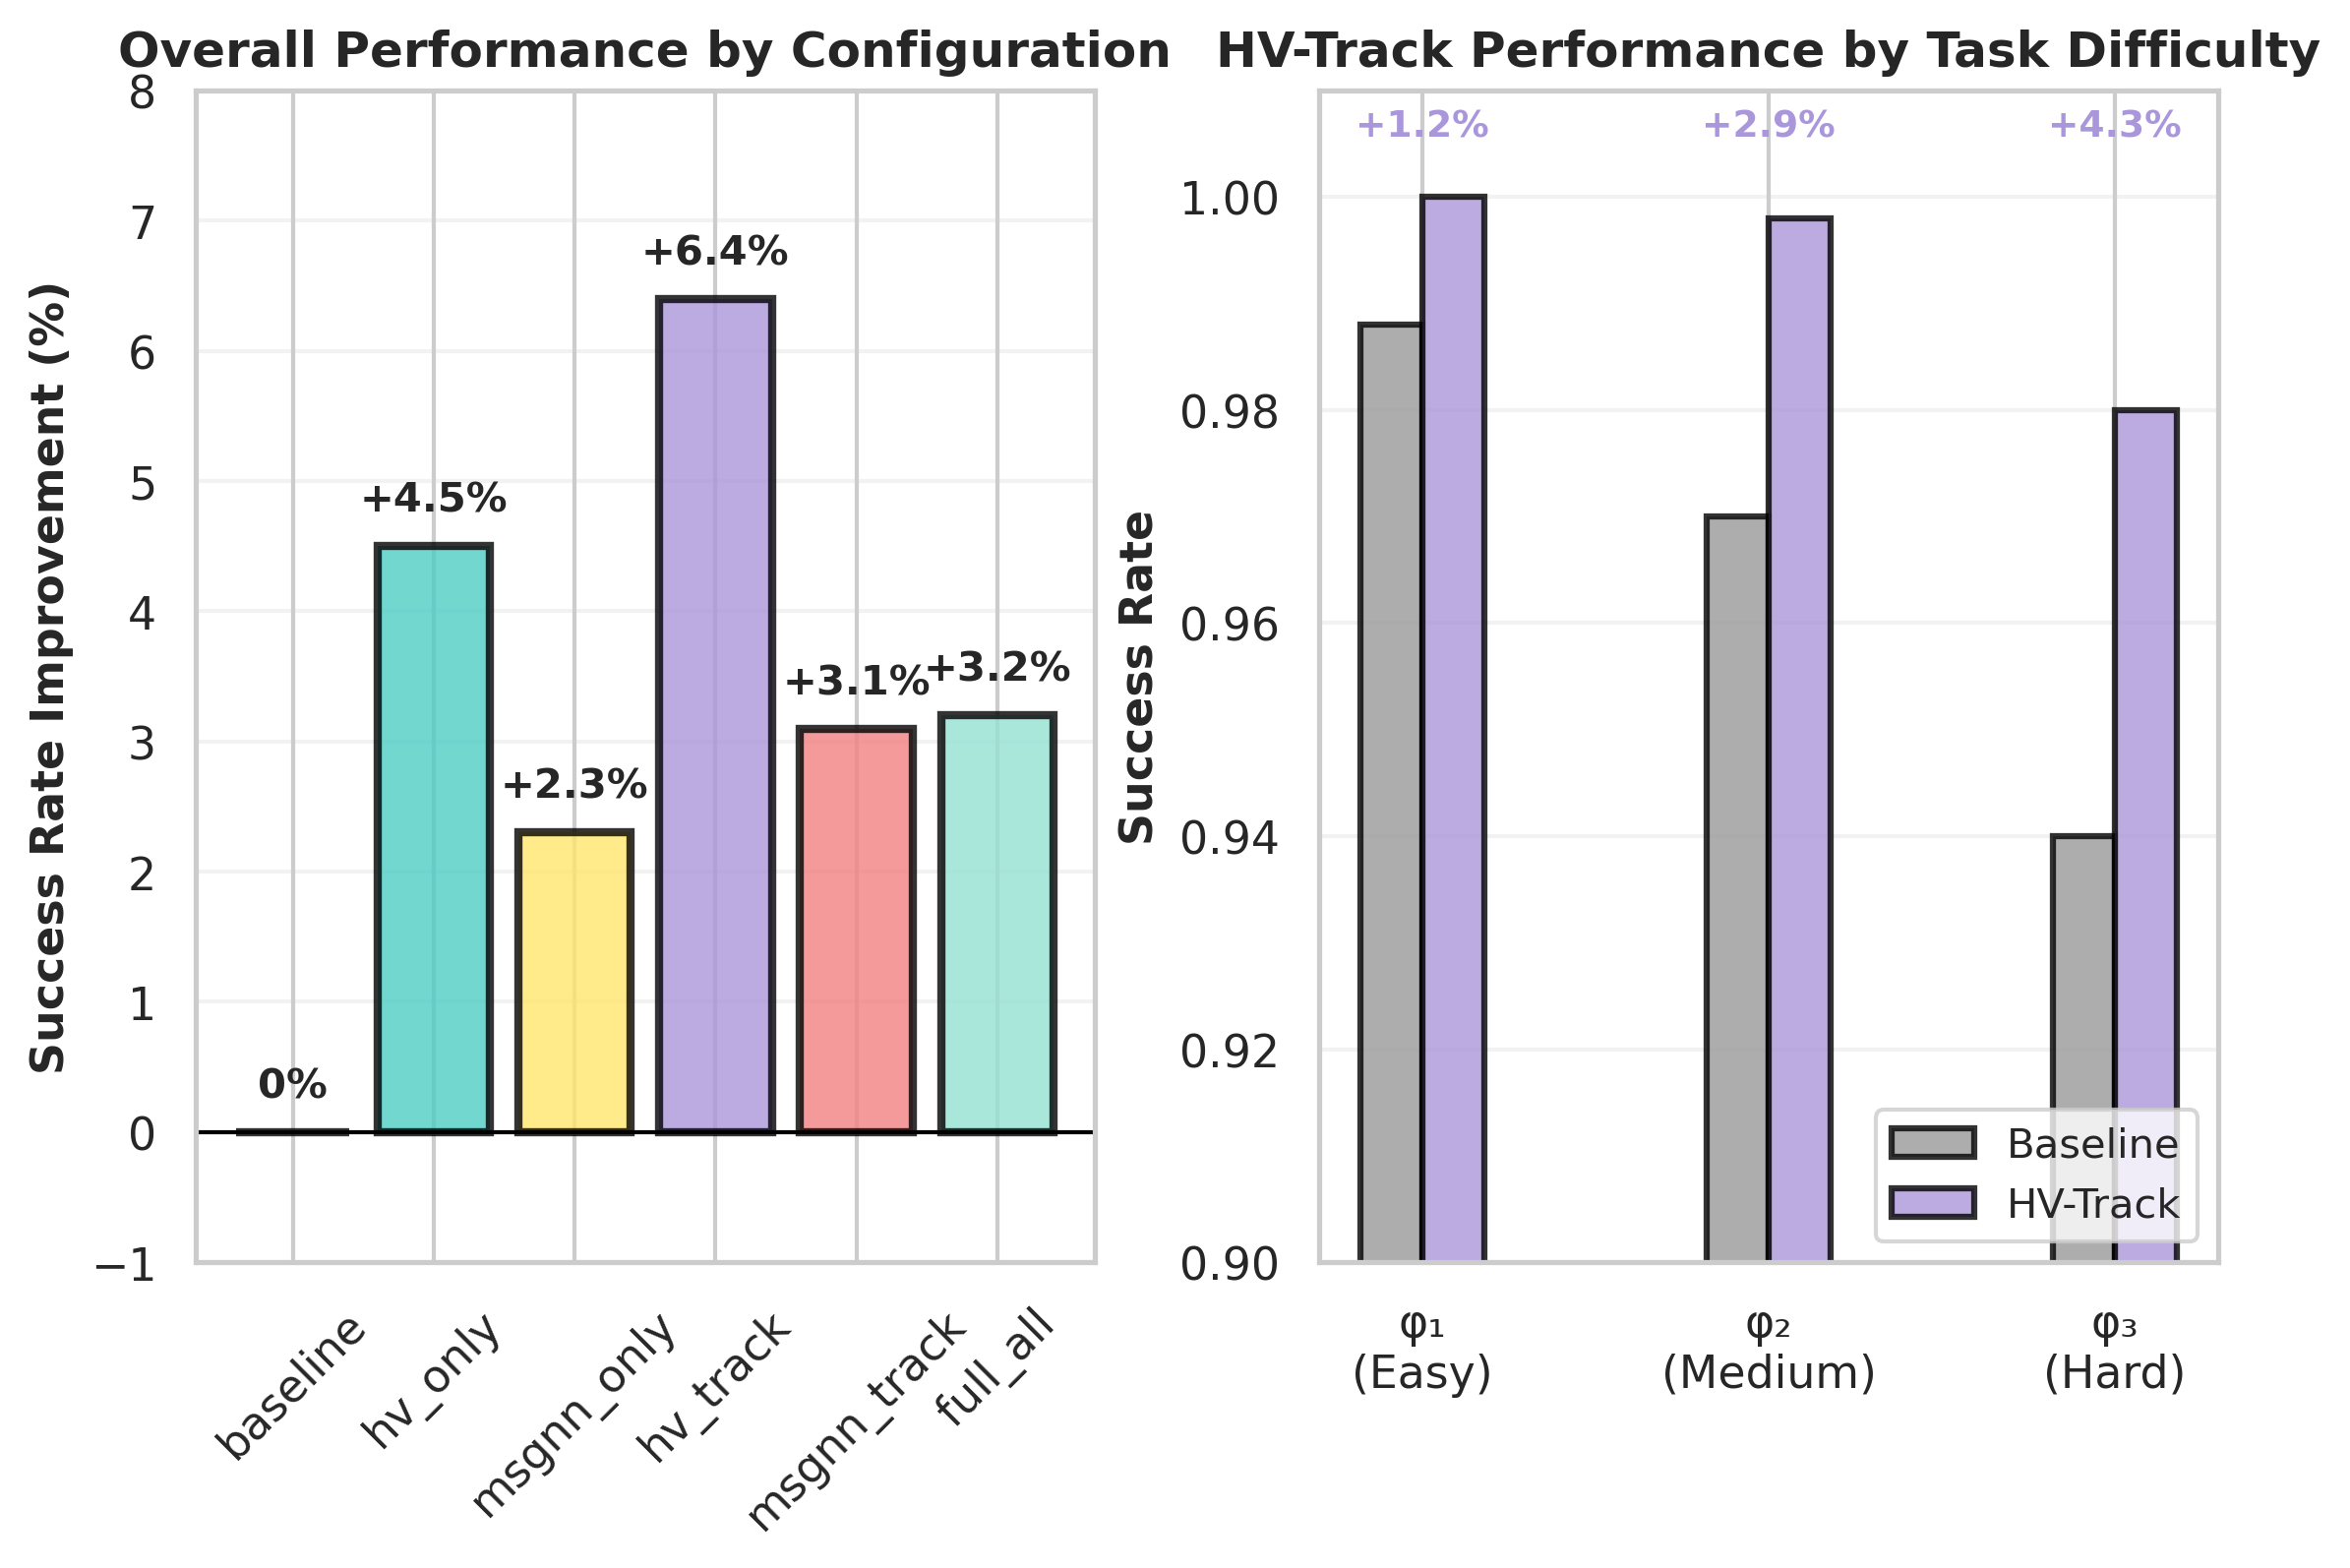
\includegraphics[width=0.95\linewidth]{figure5_performance.png}
\caption{Reported SR comparisons. \textbf{Left:} relative aggregate gains over baseline are +4.5\% (hv\_only), +2.3\% (msgnn\_only), +6.4\% (hv\_track), +3.1\% (msgnn\_track), and +3.2\% (full\_all). \textbf{Right:} task-level annotations for hv\_track are +1.2\%, +2.9\%, and +4.3\%. The two panels are reported separately; the right-panel annotations are not averaged to obtain the left-panel aggregate.}
\label{fig:performance}
\end{figure*}

\subsection{Cross-Environment Performance}

We provide a cross-environment view over ZoneEnv, LetterEnv, and FlatWorld. Table~\ref{tab:cross_env} reports averaged SR over three representative finite-horizon formulas per environment.

Both hv\_only and hv\_track outperform the internal baseline across the three environments. The hv\_track variant has the higher SR on ZoneEnv and LetterEnv, while hv\_only is slightly higher on FlatWorld (0.978 versus 0.976). Averaging the displayed environment-level SRs gives 0.984 for hv\_track, compared with 0.943 for the internal baseline, 0.743 for LTL2Action, and 0.877 for GCRL-LTL. These comparisons show positive mean performance differences across the tested environments.

\begin{table*}[t]
\centering
\caption{Cross-Environment Success Rate Comparison (Finite-horizon)}
\label{tab:cross_env}
\begin{tabular}{@{}lcccc@{}}
\toprule
\textbf{Method} & \textbf{ZoneEnv} & \textbf{LetterEnv} & \textbf{FlatWorld} & \textbf{Avg SR} \\ \midrule
LTL2Action & 0.717 & 0.622 & 0.890 & 0.743 \\
GCRL-LTL & 0.873 & 0.940 & 0.818 & 0.877 \\
baseline (internal) & 0.933 & 0.941 & 0.956 & 0.943 \\
hv\_only (internal) & 0.975 & 0.971 & \textbf{0.978} & 0.975 \\
hv\_track (internal) & \textbf{0.993} & \textbf{0.984} & 0.976 & \textbf{0.984} \\ \bottomrule
\end{tabular}
\end{table*}

\subsection{Recurrent and Persistence Objectives}

Figure~\ref{fig:zoneenv_vis} provides finite trajectory excerpts for $GF\,\mathrm{blue}\land GF\,\mathrm{yellow}$ and $FG\,\mathrm{green}$. The first objective requires repeated visits to both colors; the second requires eventual permanent residence in green. These excerpts illustrate observed behavior within a finite window. They do not establish infinite-trace satisfaction or an infinite-horizon success probability.

\subsection{Impact of Task Difficulty on Hierarchical Value Networks}

The task-level annotations in Figure~\ref{fig:performance} report positive gains for hv\_track on the three displayed tasks: +1.2\% on $\varphi_1$, +2.9\% on $\varphi_2$, and +4.3\% on $\varphi_3$. The largest displayed gain occurs on constrained reachability. Formula structure and automaton size both vary across these examples, so this comparison does not isolate an effect of automaton size. Steps and rewards are reported separately in Table~\ref{tab:hv-steps-rewards}.

Table~\ref{tab:hv_comparison} reports aggregate configuration comparisons. The component-removal study in Section~\ref{app:ablation} separately examines the contribution of the value network, tracking, and fusion on $\varphi_3$.



The aggregate relative SR gains are +4.5\% for hv\_only and +6.4\% for hv\_track. The full\_all reference gives +3.2\%, while full\_no\_options is 0.4\% below baseline. Since full\_all also enables Options, its comparison with hv\_track does not isolate MSGNN. The highest reported aggregate SR is obtained by hv\_track. The results motivate further controlled comparisons of component interactions rather than establishing a general interference mechanism.

\subsection{Hierarchical Value Effectiveness}

Three design choices motivate the hierarchical critic. First, the two heads use TD and MC supervision for discounted return; the reported aggregate SR rises from 93.3\% for baseline to 99.3\% for hv\_track. Second, the long head combines environmental state, logical state, and optional history; the component-removal comparison reports a 1.0 percentage-point reduction without tracking. Third, the fixed gate increases from approximately 0.1824 at $p=0$ to 0.8176 at $p=1$, with $\beta=0.5$ at $p=0.5$. Removing dynamic fusion reduces the reported single-task SR by 0.5 percentage points. These observations are consistent with a benefit from the tested design choices, but do not establish a unique causal explanation.

\begin{figure*}[ht]
\centering
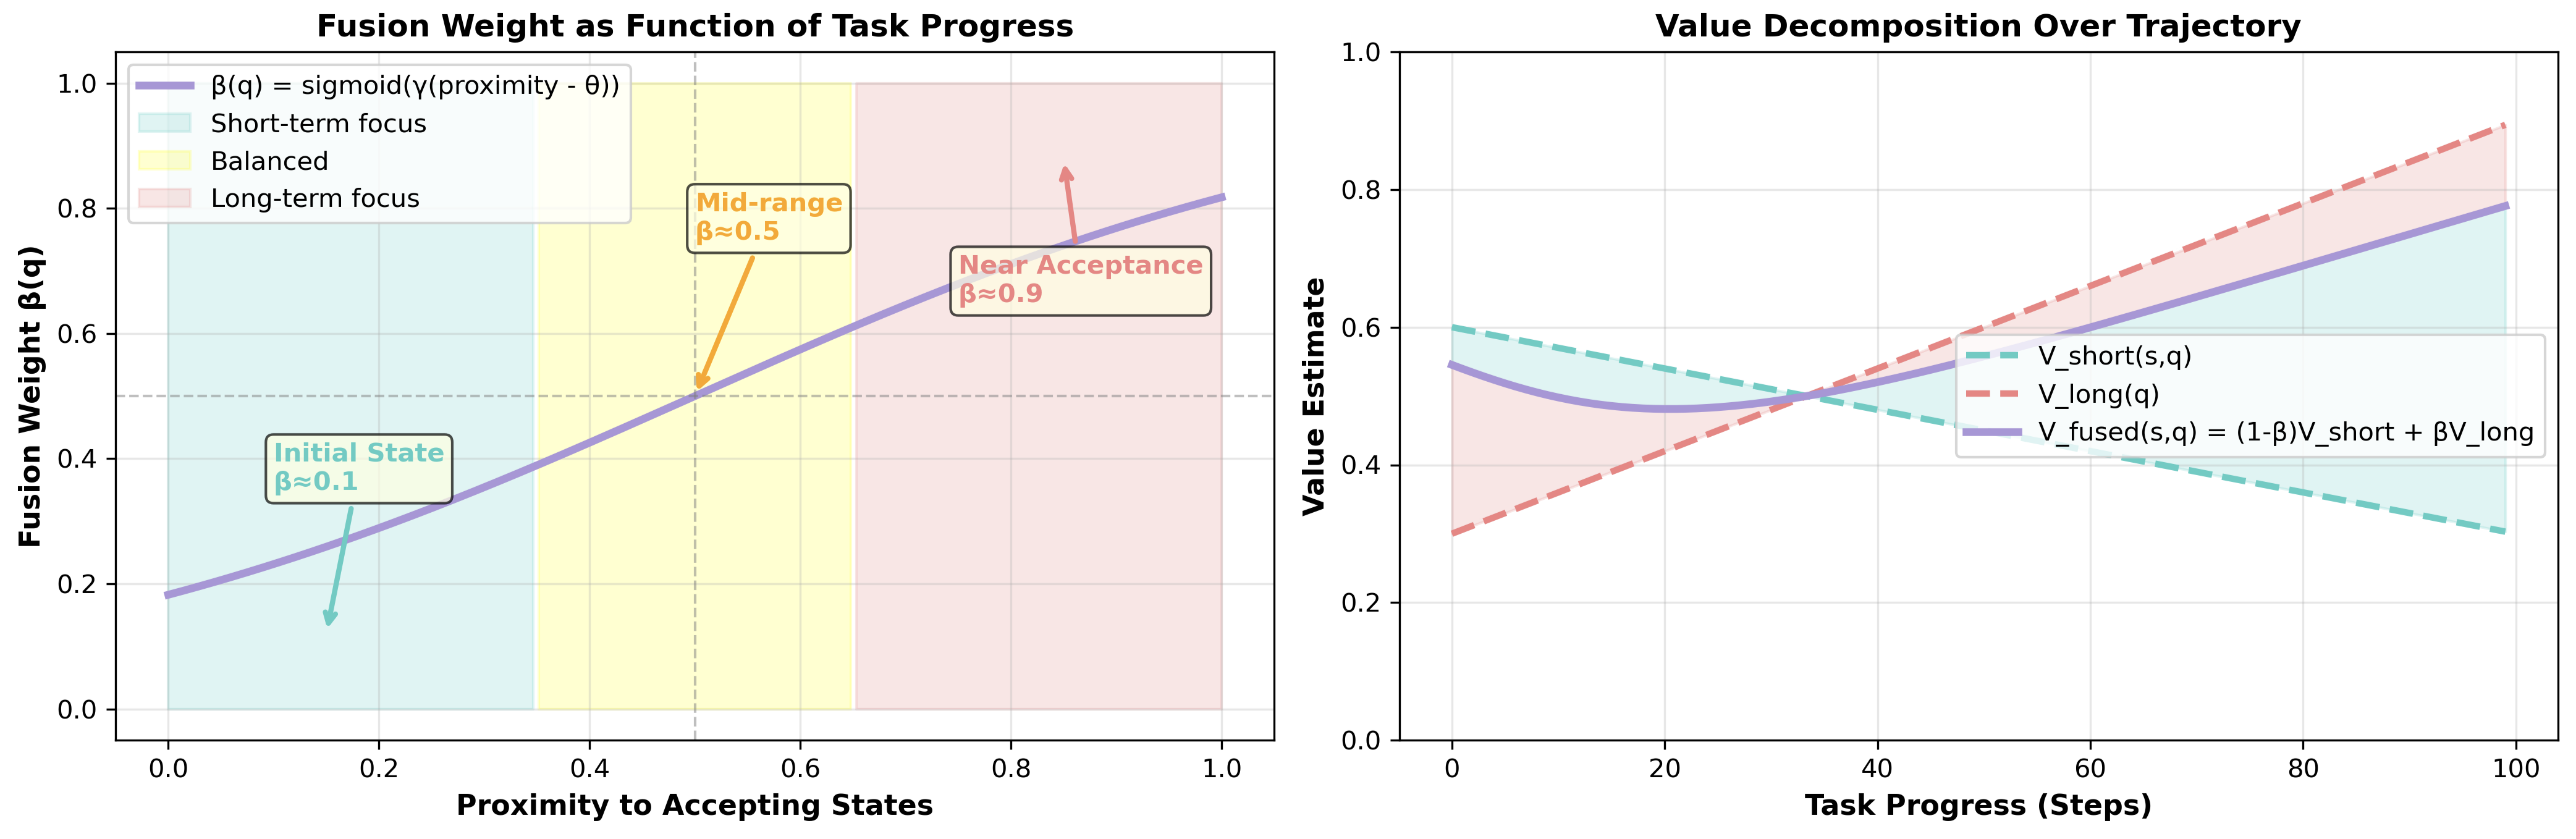
\includegraphics[width=0.95\linewidth]{figure4_fusion_weight.png}
\caption{Illustration of progress-dependent fusion. \textbf{Left:} the plotted sigmoid corresponds to $\beta=\sigma(3(p-0.5))$, with values approximately 0.1824, 0.5, and 0.8176 at $p=0$, $0.5$, and $1$. The slope symbol $\gamma$ in the image denotes $\kappa$, separate from the RL discount. \textbf{Right:} illustrative value pathways and their convex fusion over a trajectory; $V_{\mathrm{long}}(q)$ suppresses environmental and optional history arguments. The value curves illustrate the fusion rule and are not an empirical convergence analysis.}
\label{fig:fusion_weight}
\end{figure*}

\begin{table}[t]
\centering
\caption{Summary of Component Contributions (quantitative details in referenced tables)}
\label{tab:key_findings}
\small
\begin{tabular}{@{}>{\raggedright\arraybackslash}p{0.28\linewidth}>{\raggedright\arraybackslash}p{0.64\linewidth}@{}}
\toprule
\textbf{Component} & \textbf{Key Result (Source)} \\ \midrule
SE-GNN & Semantic feature design (Eqs.~\ref{eq:node_features}--\ref{eq:edge_features}) \\
Hierarchical Value & Main configuration gains (Table~\ref{tab:hv_comparison}) \\
Dynamic Fusion & Component ablation (Table~\ref{tab:ablation}) \\
Automaton Tracking & Component ablation (Table~\ref{tab:ablation}) \\
Task Difficulty & Comparison on the tested tasks (Figure~\ref{fig:performance}) \\ \bottomrule
\end{tabular}
\end{table}

\begin{table*}[t]
\centering
\caption{Reported Aggregate Performance on PointLtl2-v0. Internal results use 500 episodes per seed, averaged over seeds 1--5. External baseline values are historical references; their original task suite and protocol differ from the internal comparison. Relative gains are computed from the displayed aggregate SRs and rounded to one decimal place.}
\label{tab:overall_performance}
\begin{tabular}{@{}lcccc@{}}
\toprule
\textbf{Model} & \textbf{Avg SR} & \textbf{Relative gain} & \textbf{Avg Steps} & \textbf{Avg Reward} \\ \midrule
LTL2Action & 0.717 & --- & 232.2 & 0.589 \\
GCRL-LTL & 0.873 & --- & 233.5 & 0.595 \\ \midrule
baseline & 0.933 & --- & 231.3 & 0.618 \\
hv\_only & 0.975 & +4.5\% & 236.8 & 0.652 \\
msgnn\_only & 0.954 & +2.3\% & 240.3 & 0.636 \\
hv\_track & \textbf{0.993} & \textbf{+6.4\%} & 235.5 & \textbf{0.663} \\
msgnn\_track & 0.962 & +3.1\% & 241.8 & 0.630 \\
full\_no\_options & 0.929 & -0.4\% & 245.2 & 0.602 \\
full\_all & 0.963 & +3.2\% & 243.1 & 0.648 \\ \bottomrule
\end{tabular}
\end{table*}

\subsection{Detailed Metrics and Component Ablations}
\label{sec:extended_ablation}

\subsubsection{Performance Metrics Details}

We analyze detailed metrics (steps and rewards) across configurations to understand the quality-versus-efficiency trade-off. Table~\ref{tab:hv-steps-rewards} reports average steps and rewards for three HV-related configurations.

\begin{table*}[t]
\centering
\caption{HV Impact on Average Steps and Rewards}
\label{tab:hv-steps-rewards}
\begin{tabular}{@{}lcccccc@{}}
	\toprule
	\textbf{Configuration} & \textbf{$\varphi_1$ Steps} & \textbf{$\varphi_2$ Steps} & \textbf{$\varphi_3$ Steps} & \textbf{Avg Steps} & \textbf{$\varphi_3$ Reward} & \textbf{Avg Reward} \\ \midrule
baseline & 197.5 & 294.5 & 201.9 & 231.3 & 0.635 & 0.618 \\
hv\_only & 209.4 & 300.2 & 200.9 & 236.8 & 0.652 & 0.652 \\
hv\_track & 196.8 & 302.3 & 207.4 & 235.5 & 0.654 & 0.663 \\ \bottomrule
\end{tabular}
\end{table*}

The reported aggregate average reward increases from 0.618 to 0.663, a relative improvement of approximately 7.3\%. The corresponding mean step counts are 231.3 and 235.5, an increase of approximately 1.8\%. On $\varphi_3$, the reported mean step count increases from 201.9 to 207.4, a difference of 5.5 steps. These means describe a reward--step trade-off; they do not establish a reduction in trajectory variance or identify the cause of individual successes.

\subsubsection{Component Ablation Study}
\label{app:ablation}

To isolate the contribution of each architectural component, we conduct systematic ablation experiments based on the best-performing hv\_track configuration.

\begin{table}[h]
\centering
\caption{Ablation Study (based on hv\_track)}
\label{tab:ablation}
\begin{tabular}{@{}lccc@{}}
	\toprule
	\textbf{Removed Component} & \textbf{$\varphi_3$ SR} & \textbf{$\Delta$ SR (pp)} & \textbf{Avg Reward} \\ \midrule
Complete (hv\_track) & 0.980 & --- & 0.654 \\
- HV network & 0.962 & -1.8 & 0.635 \\
- Automaton Tracking & 0.970 & -1.0 & 0.644 \\
- Dynamic fusion ($\beta(q)$) & 0.975 & -0.5 & 0.650 \\ \bottomrule
\end{tabular}
\end{table}

The component-removal results are reported for $\varphi_3$ using the stated PPO budget and learning rate. Each row removes the named mechanism from hv\_track. These comparisons are separate from the aggregate configuration comparison.

The component-removal results in Table~\ref{tab:ablation} show SR reductions of 1.8, 1.0, and 0.5 percentage points when the HV network, automaton tracking, and dynamic fusion are removed, respectively. The largest reduction in this comparison follows removal of the HV network. These single-task component-removal effects are distinct from the aggregate configuration gains in Table~\ref{tab:hv_comparison}.



\section{Conclusion}
\label{sec:conclusion}

HiLTL combines semantic automaton representations, TD- and MC-supervised value pathways, and progress-dependent fusion. The reported aggregate ZoneEnv comparison gives a +6.4\% relative SR gain for hv\_track over the internal baseline. Cross-environment means and the single-task component-removal study provide complementary descriptive comparisons. The trajectory illustrations demonstrate behavior under recurrent and persistence objectives within finite windows. The results motivate hierarchical value learning for the tested logic-conditioned control tasks; they do not provide a formal guarantee of satisfaction or safety.

The best reported aggregate result is obtained by hv\_track, while the additional value of multi-layer pooling depends on configuration. Future work should test larger automata, specify controlled component interventions, and measure computational cost under matched training budgets. These evaluations are needed before making general claims about scalability or architectural interactions.





% if have a single appendix:
%\appendix[Proof of the Zonklar Equations]
% or
%\appendix  % for no appendix heading
% do not use \section anymore after \appendix, only \section*
% is possibly needed

% use appendices with more than one appendix
% then use \section to start each appendix
% you must declare a \section before using any
% \subsection or using \label (\appendices by itself
% starts a section numbered zero.)
%


\appendices

\section{Algorithm Specifications}
\label{app:algorithms}

This appendix provides detailed algorithmic specifications of HiLTL's three core components: SE-GNN construction, hierarchical value decomposition, and the complete training procedure.

\subsection{SE-GNN: Semantically-Enhanced Graph Construction}

Algorithm~\ref{alg:segnn} describes how we construct the enhanced automaton graph with semantic features.

\begin{algorithm}[h]
\caption{SE-GNN Graph Construction}
\label{alg:segnn}
\begin{algorithmic}[1]
\REQUIRE LDBA $\mathcal A=(Q,2^{AP},\delta,q_0,F_E)$
\ENSURE Graph $(V,E,X_v,X_e)$ and transition guards
\STATE $E\gets$ the directed transitions of $\mathcal A$
\STATE $Q_F\gets\{q':(q,\ell,q')\in F_E\}$
\STATE Compute SCCs of the directed graph
\STATE $d\gets$ reverse multi-source BFS from $Q_F$; unreachable distances are $\infty$
\STATE $D\gets\max(1,\max_{q:d(q)<\infty}d(q))$; inner empty maximum is zero
\STATE $\bar d(q)\gets\min\{d(q),D\}/D$ for all $q$
\FOR{each state $q\in Q$}
 \STATE $is\_target\gets\mathbb I(q\in Q_F)$
 \STATE $has\_cycle\gets\mathbb I(\text{SCC size}>1\text{ or a self-loop exists})$
 \STATE $is\_initial\gets\mathbb I(q=q_0)$
 \STATE $X_v[q]\gets[is\_target,has\_cycle,is\_initial,\bar d(q)]$
\ENDFOR
\FOR{each edge $e=(q,\ell,q')\in E$}
 \STATE $edge\_type\gets$ ClassifyTransition$(e,d)$, testing epsilon first
 \STATE $type\_onehot\gets$ OneHot$(edge\_type,4)$
\STATE Use order [progress, remaining, reserved, epsilon]
 \STATE $X_e[e]\gets[type\_onehot,\mathbb I(q'\in Q_F),\bar d(q')]$
 \STATE Retain the guard for separate encoding
\ENDFOR
\STATE \textbf{return} $(V=Q,E,X_v,X_e)$ and guards
\end{algorithmic}
\end{algorithm}

\textbf{Edge Type Classification.} For $e=(q,\ell,q')$, the classifier uses the following ordered rules:
\begin{itemize}
\item \texttt{epsilon}: the edge is an epsilon choice.
\item \texttt{progress}: a non-epsilon edge with $d(q')<d(q)$.
\item \texttt{remaining}: any other non-epsilon edge, including self-loops and equal-distance edges.
\end{itemize}
The skip slot is reserved and zero; no real edge is classified by a shortest-hop decrease greater than one.

\subsection{Hierarchical Value Decomposition with Dynamic Fusion}

Algorithm~\ref{alg:hv} presents the hierarchical value computation during policy evaluation.

\begin{algorithm}[h]
\caption{Hierarchical Value Estimation}
\label{alg:hv}
\begin{algorithmic}[1]
\REQUIRE State $s_t$, logical state $q_t$, graph embeddings, optional history $H_t$
\REQUIRE Value networks $V_{\mathrm{short}},V_{\mathrm{long}}$; fixed $\kappa=3,\theta=0.5$
\ENSURE Fused value and pathway estimates
\STATE $p\gets1-\bar d(q_t)$
\STATE $v_s\gets V_{\mathrm{short}}(s_t,q_t)$ using the short-head representation
\IF{tracking is enabled}
 \STATE $h_H\gets\operatorname{LSTM}(\mathbf h_{q_0},\ldots,\mathbf h_{q_t})$
  \STATE $v_l\gets\operatorname{MLP}_{\mathrm{long}}([\mathbf s_t;p;\mathbf h_{q_t};h_H])$
\ELSE
  \STATE $v_l\gets\operatorname{MLP}_{\mathrm{long}}([\mathbf s_t;p;\mathbf h_{q_t}])$
\ENDIF
\STATE $\beta\gets\sigma(\kappa(p-\theta))$
\STATE $V_{\mathrm{total}}\gets(1-\beta)v_s+\beta v_l$
\STATE \textbf{return} $V_{\mathrm{total}},\{v_s,v_l,\beta\}$
\end{algorithmic}
\end{algorithm}

\textbf{Intuition:} The MC-supervised long head receives weight approximately 0.1824 at zero proximity, 0.5 at medium proximity, and 0.8176 at unit proximity. The rule is fixed in parameter space and varies with logical state. Proximity need not increase monotonically within an episode.

\subsection{Complete Training Procedure}

Algorithm~\ref{alg:training} summarizes training with a reach--avoid curriculum and vectorized PPO rollouts. The logical context $C_t$ includes the sampled sequence monitor, current logical state, and optional visited-state history. At evaluation, the test formula is translated to an LDBA and the inherited sequence-selection procedure supplies policy conditioning. Training monitors and test-formula automata therefore have different roles. The trainable parameters are denoted $\Theta$, distinct from the fixed gate threshold $\theta$.

\begin{algorithm}[t]
\caption{HiLTL Training with TD/MC Value Supervision}
\label{alg:training}
\begin{algorithmic}[1]
\REQUIRE Environment, reach--avoid curriculum, rollout budget
\REQUIRE $\lambda_{\mathrm{short}}=1$, $\lambda_{\mathrm{long}}=0.3$
\ENSURE Policy and value-network parameters $\Theta$
\STATE Initialize policy, graph encoder, and enabled value heads
\STATE Set fixed gate constants $\kappa=3$, $\theta=0.5$
\STATE Initialize parallel environments and per-environment episode buffers
\WHILE{the training budget remains}
 \STATE Sample curriculum tasks at environment resets
 \STATE Construct their sequence monitors and semantic graphs
 \STATE Collect a vectorized rollout with the current policy
 \STATE Use environment, sequence, and enabled graph context for actions
 \STATE Handle enabled epsilon choices through the logical wrapper
 \STATE Store rewards, actions, old log probabilities, values, and context
 \STATE Update logical history on interaction steps; reset at episode boundaries
 \STATE Compute PPO advantages and returns using the fused critic
 \STATE Clip actor advantages to $[-1,1]$ under the reported protocol
 \STATE Compute fixed short-head targets with collection-time parameters:
 \STATE $y_t\gets r_t+\gamma_{\mathrm{RL}}(1-m_t)V_{\mathrm{short,old}}(s_{t+1},q_{t+1})$
 \STATE For completed episodes, compute $G_t$ by discounted backward accumulation
 \STATE Retain unfinished episode buffers for subsequent collection
 \FOR{each PPO epoch and minibatch}
  \STATE Recompute trainable graph and history representations
  \STATE Evaluate the policy and enabled value heads
  \STATE $\mathcal L_s\gets\operatorname{mean}_t(V_{\mathrm{short},t}-y_t)^2$
  \STATE $\mathcal L_l\gets\operatorname{mean}_t(V_{\mathrm{long},t}-G_t)^2$
  \STATE Use $\mathcal L_l=0$ if no completed-episode examples exist
  \STATE Compute clipped PPO actor and fused-critic losses
  \STATE $\mathcal L\gets\mathcal L_{\mathrm{PPO}}+\lambda_{\mathrm{short}}\mathcal L_s+\lambda_{\mathrm{long}}\mathcal L_l$
  \STATE Update $\Theta$ with Adam; invalidate cached embeddings
 \ENDFOR
 \STATE Discard consumed completed-episode MC examples
\ENDWHILE
\STATE \textbf{return} $\Theta$
\end{algorithmic}
\end{algorithm}

The auxiliary losses apply when HV is enabled. The long head receives environmental and logical context, with optional history, as specified in Algorithm~\ref{alg:hv}. Both heads predict discounted return. Here $m_t=1$ at a defined episode boundary, including the finite task horizon, and $m_t=0$ otherwise; rollout boundaries alone do not end an episode. Incomplete episodes are not assigned zero MC targets. Completed episodes may span policy updates, so their MC returns need not have been collected under one frozen policy. The gate constants are fixed and are distinct from the RL reward discount.


\section{Future Directions for MSGNN}
\label{app:future_directions}

The configuration comparisons in Section~\ref{sec:extended_ablation} motivate the following research directions. They are proposed evaluations, not completed experiments or quantitative performance forecasts.

\subsection{Direction 1: Larger Automata}

Evaluate richer proposition sets, nested formulas, and safety--liveness combinations. Record automaton size and structure after a fixed translation and pruning protocol. Graph encoders~\citep{Kipf2017,wang2023graph} provide candidate architectures, while probabilistic modeling~\citep{murphy2018machine} offers complementary perspectives. Their performance on these tasks should be measured under matched budgets; graph size alone does not determine the required message-passing depth.

\subsection{Direction 2: Architecture and Cost}

Compare GNN depth, attention heads, hidden dimensions, and pooling operators with multiple independent training seeds. Report parameter counts, training time, inference latency, and performance. Offline meta-RL~\citep{pong2022offline} is a separate possible adaptation direction and is not evaluated here.

\subsection{Direction 3: Semantic Features}

Transition guards and acceptance-target distances are already represented. Future ablations should test richer interactions between guard semantics and graph structure, recurrent-acceptance information, and logical implication features. Such comparisons should separate feature contributions from additional model capacity.

\subsection{Direction 4: Co-Design with Value Learning}

Investigate how representations at different message-passing depths should condition the value pathways. Three-hop context is not necessarily global context. Vary MSGNN, Options, and value-pathway routing separately: full\_all changes more than one component relative to hv\_track, so their performance difference cannot identify a unique interaction. No numerical improvement is predicted before these comparisons are performed.



% Can use something like this to put references on a page
% by themselves when using endfloat and the captionsoff option.
\ifCLASSOPTIONcaptionsoff
  \newpage
\fi



% trigger a \newpage just before the given reference
% number - used to balance the columns on the last page
% adjust value as needed - may need to be readjusted if
% the document is modified later
%\IEEEtriggeratref{8}
% The "triggered" command can be changed if desired:
%\IEEEtriggercmd{\enlargethispage{-5in}}

% references section

% can use a bibliography generated by BibTeX as a .bbl file
% BibTeX documentation can be easily obtained at:
% http://mirror.ctan.org/biblio/bibtex/contrib/doc/
% The IEEEtran BibTeX style support page is at:
% http://www.michaelshell.org/tex/ieeetran/bibtex/
\bibliographystyle{IEEEtranN}
% argument is your BibTeX string definitions and bibliography database(s)
\bibliography{ref}
%
% <OR> manually copy in the resultant .bbl file
% set second argument of \begin to the number of references
% (used to reserve space for the reference number labels box)
%\begin{thebibliography}{1}

%\bibitem{IEEEhowto:kopka}
%H.~Kopka and P.~W. Daly, \emph{A Guide to \LaTeX}, 3rd~ed.\hskip 1em plus
%  0.5em minus 0.4em\relax Harlow, England: Addison-Wesley, 1999.

%\end{thebibliography}

% biography section
% 
% If you have an EPS/PDF photo (graphicx package needed) extra braces are
% needed around the contents of the optional argument to biography to prevent
% the LaTeX parser from getting confused when it sees the complicated
% \includegraphics command within an optional argument. (You could create
% your own custom macro containing the \includegraphics command to make things
% simpler here.)
%\begin{IEEEbiography}[{\includegraphics[width=1in,height=1.25in,clip,keepaspectratio]{mshell}}]{Michael Shell}
% or if you just want to reserve a space for a photo:


% You can push biographies down or up by placing
% a \vfill before or after them. The appropriate
% use of \vfill depends on what kind of text is
% on the last page and whether or not the columns
% are being equalized.

%\vfill

% Can be used to pull up biographies so that the bottom of the last one
% is flush with the other column.
%\enlargethispage{-5in}



% that's all folks
\end{document}


